\section{Introducción}
En este capítulo se explica la estructura del código del proyecto, tanto en la parte del \textit{frontend} en Angular como en la parte del \textit{backend} con NodeJS. Además, se explican los principales problemas encontrados durante el desarrollo del proyecto y los diferentes tipos de pruebas realizadas para comprobar el correcto funcionamiento de la aplicación Web.




\section{Estructura del código de \textit{frontend}}
En esta sección se detalla la estructura de ficheros en la parte realizada en Angular para el \textit{frontend}. Hay ciertas carpetas en las que no se muestra su estructura debido a su similitud con otras. En la Figura \ref{fig:dirtreeAngular} se muestra esta estructura.


\begin{figure}
    \centering
    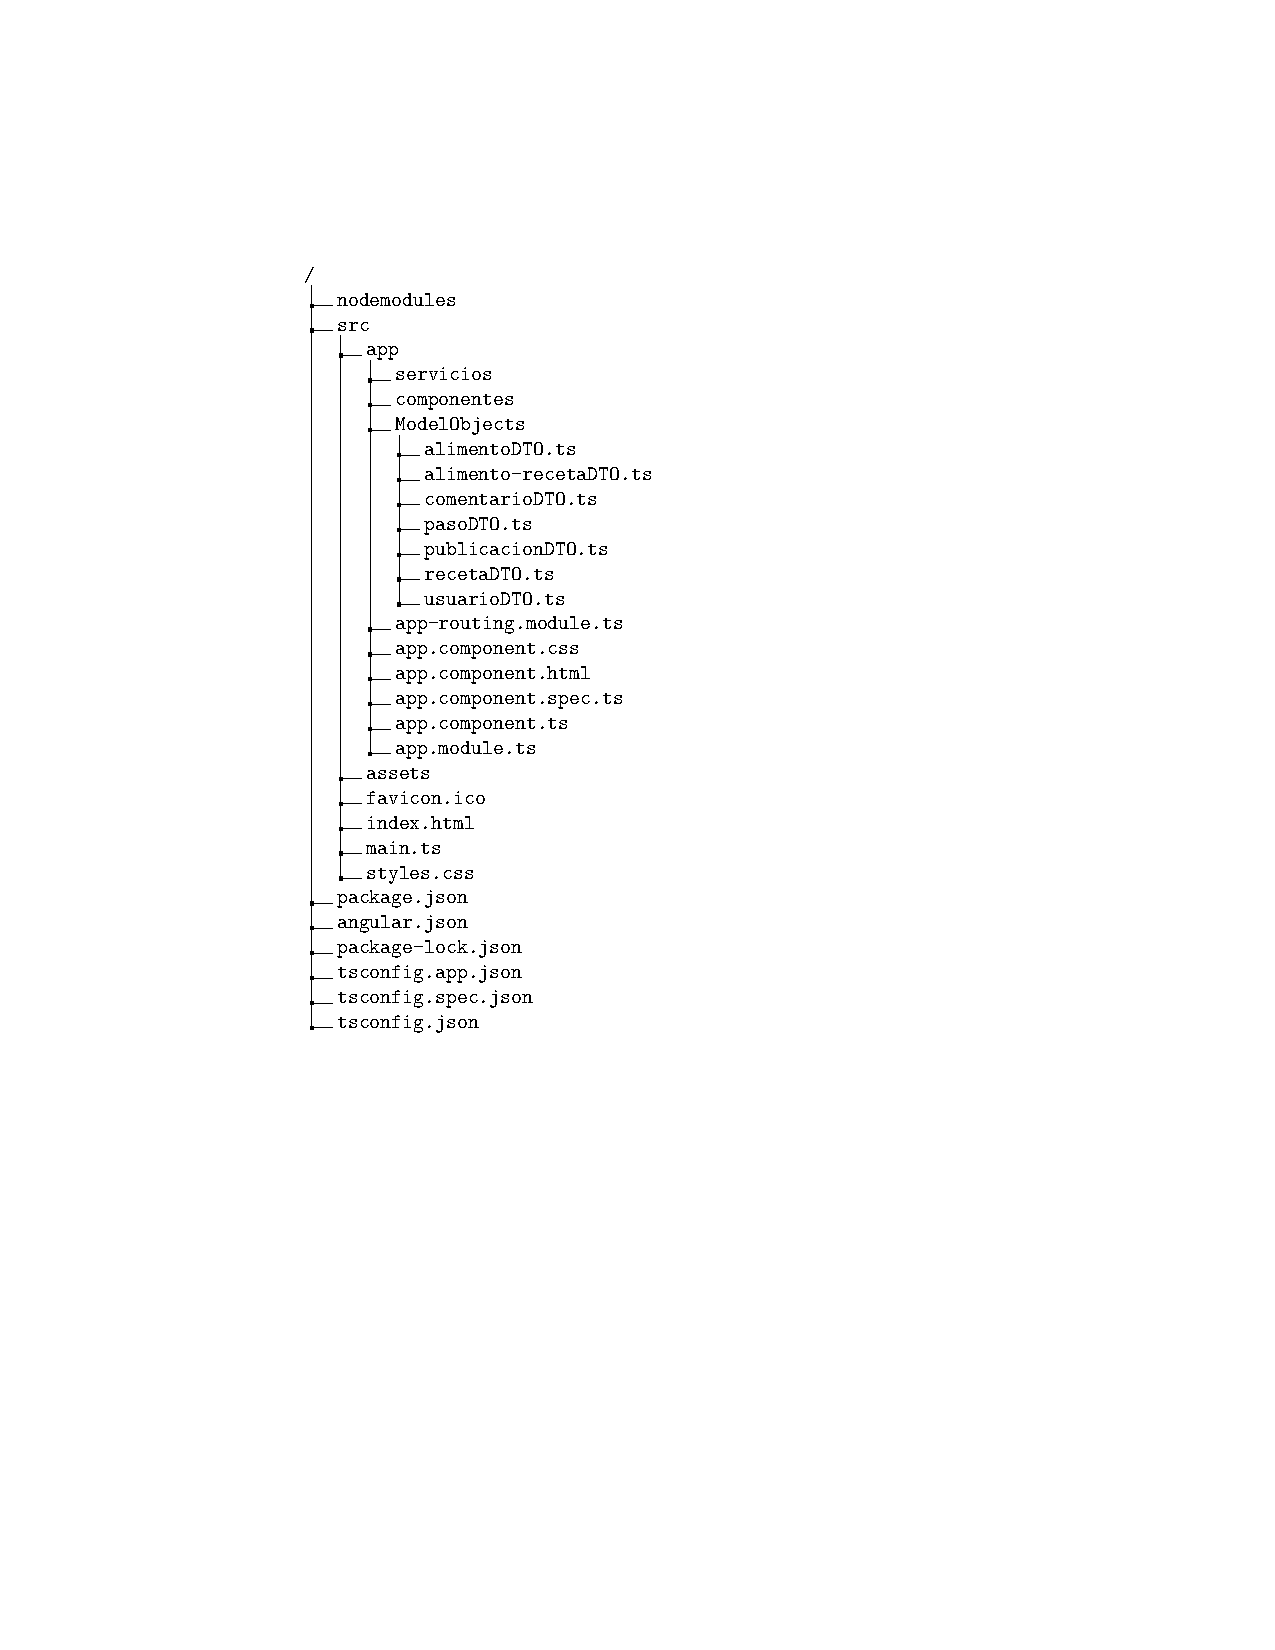
\includegraphics{svg/dirtreefront.pdf}
    \caption{Estructura de ficheros en la parte del \textit{frontend} en Angular.}
    \label{fig:dirtreeAngular}
\end{figure}

A continuación se detalla el contenido de las carpetas mostradas en esta estructura:

\begin{itemize}
    \item \texttt{nodemodules}: contiene los paquetes instalados que se usan en Angular.
    \item \texttt{app}: contiene todo el código del proyecto. Dentro de esta carpeta destacan los archivos:
    \begin{itemize}
        \item \texttt{app-routing.module.ts}: contiene las rutas de acceso para cada componente gráfico de la interfaz de la aplicación, es decir, la ruta que aparecerá en la barra del navegador para acceder a cada componente de la interfaz.
        \item \texttt{app.module.ts}: donde se importan todos los componentes de la aplicación y los módulos que se van a utilizar.
    \end{itemize}
\end{itemize}


 Además la carpeta \texttt{app} contiene tres carpetas y el contenido que almacena cada una de ellas es el siguiente:
\begin{itemize}
    \item  \texttt{ModelObjects}: que contiene los DTO utilizados para gestionar los datos introducidos por el Usuario y obtenidos del \textit{backend} en el \textit{frontend}.
        
    \item  \texttt{servicios}: contiene carpetas que almacenan los servicios que se comunicarán con el \textit{backend} para obtener la información de la base de datos y guardar cambios sobre la información almacenada en ella. Hay varios servicios, cada uno asociado a una tabla de la base de datos, y almacenarán las peticiones que se realicen al \textit{backend} y que afecten a la tabla de la base de datos asociada. Cada una de estas carpetas almacena dos archivos:
    \begin{itemize}
        \item Un archivo terminado en \texttt{service.spec.ts} que sirve para realizar test unitarios.
        \item Un archivo terminado en \texttt{service.ts} en el que se almacenan los métodos que realizan las peticiones al \textit{backend}.
    \end{itemize}
    
    
    
     
    \item  \texttt{componentes}: almacena los componentes gráficos de la interfaz de la aplicación Web. Al ser un número elevado de componentes de la interfaz, se han agrupado según su funcionalidad. La descripción de estas carpetas que se han utilizado para agrupar los componentes es la siguiente:
    \begin{itemize}
        \item \texttt{admin-vistas:} en esta carpeta se encuentran todos los componentes que podrá ver el Administrador cuando se identifique en la aplicación. 
        \item \texttt{buscadores:} contiene dos carpetas:
        \begin{itemize}
            \item \texttt{componentes-buscar:} donde se encuentran las vistas en las que se puede realizar una búsqueda de un determinado elemento. Estas interfaces son reutilizables ya que utilizadas por otros componentes.
            \item \texttt{vistas-buscar:} contiene los componentes que solo se utilizan para realizar búsquedas y por lo tanto estos componentes utilizan el componente de la carpeta \texttt{componentes-buscar} que corresponda.
        \end{itemize}

        \item \texttt{cartas:} en esta carpeta se agrupan los componentes que sirven como cartas para representar la información más relevante de una instancia de un determinado tipo de datos. Estas cartas son utilizadas por varias interfaces en la aplicación.
        \item \texttt{creadores:} en esta carpeta se pueden encontrar a las interfaces que servirán para crear un contenido por parte del Usuario y que se almacenará en la base de datos. 
        \item \texttt{detalles:} en esta carpeta se encuentran las vistas que sirven para mostrar toda la información de un elemento concreto de entre todos los tipos de datos diferentes que se manejan en la aplicación.
        \item \texttt{gestiones-usuario:} en esta carpeta se encuentran los componentes que muestran los datos almacenados del Usuario y la modificación de estos.
        \item \texttt{sin-identificar:} en esta carpeta se encuentran las vistas que serán utilizadas por los usuarios antes de que se identifiquen en la aplicación. 
    \end{itemize}
\end{itemize}



En la Figura \ref{fig:dirtreeServicios} se muestra la estructura de ficheros dentro de la carpeta \texttt{servicios}.

\begin{figure}
    \centering
    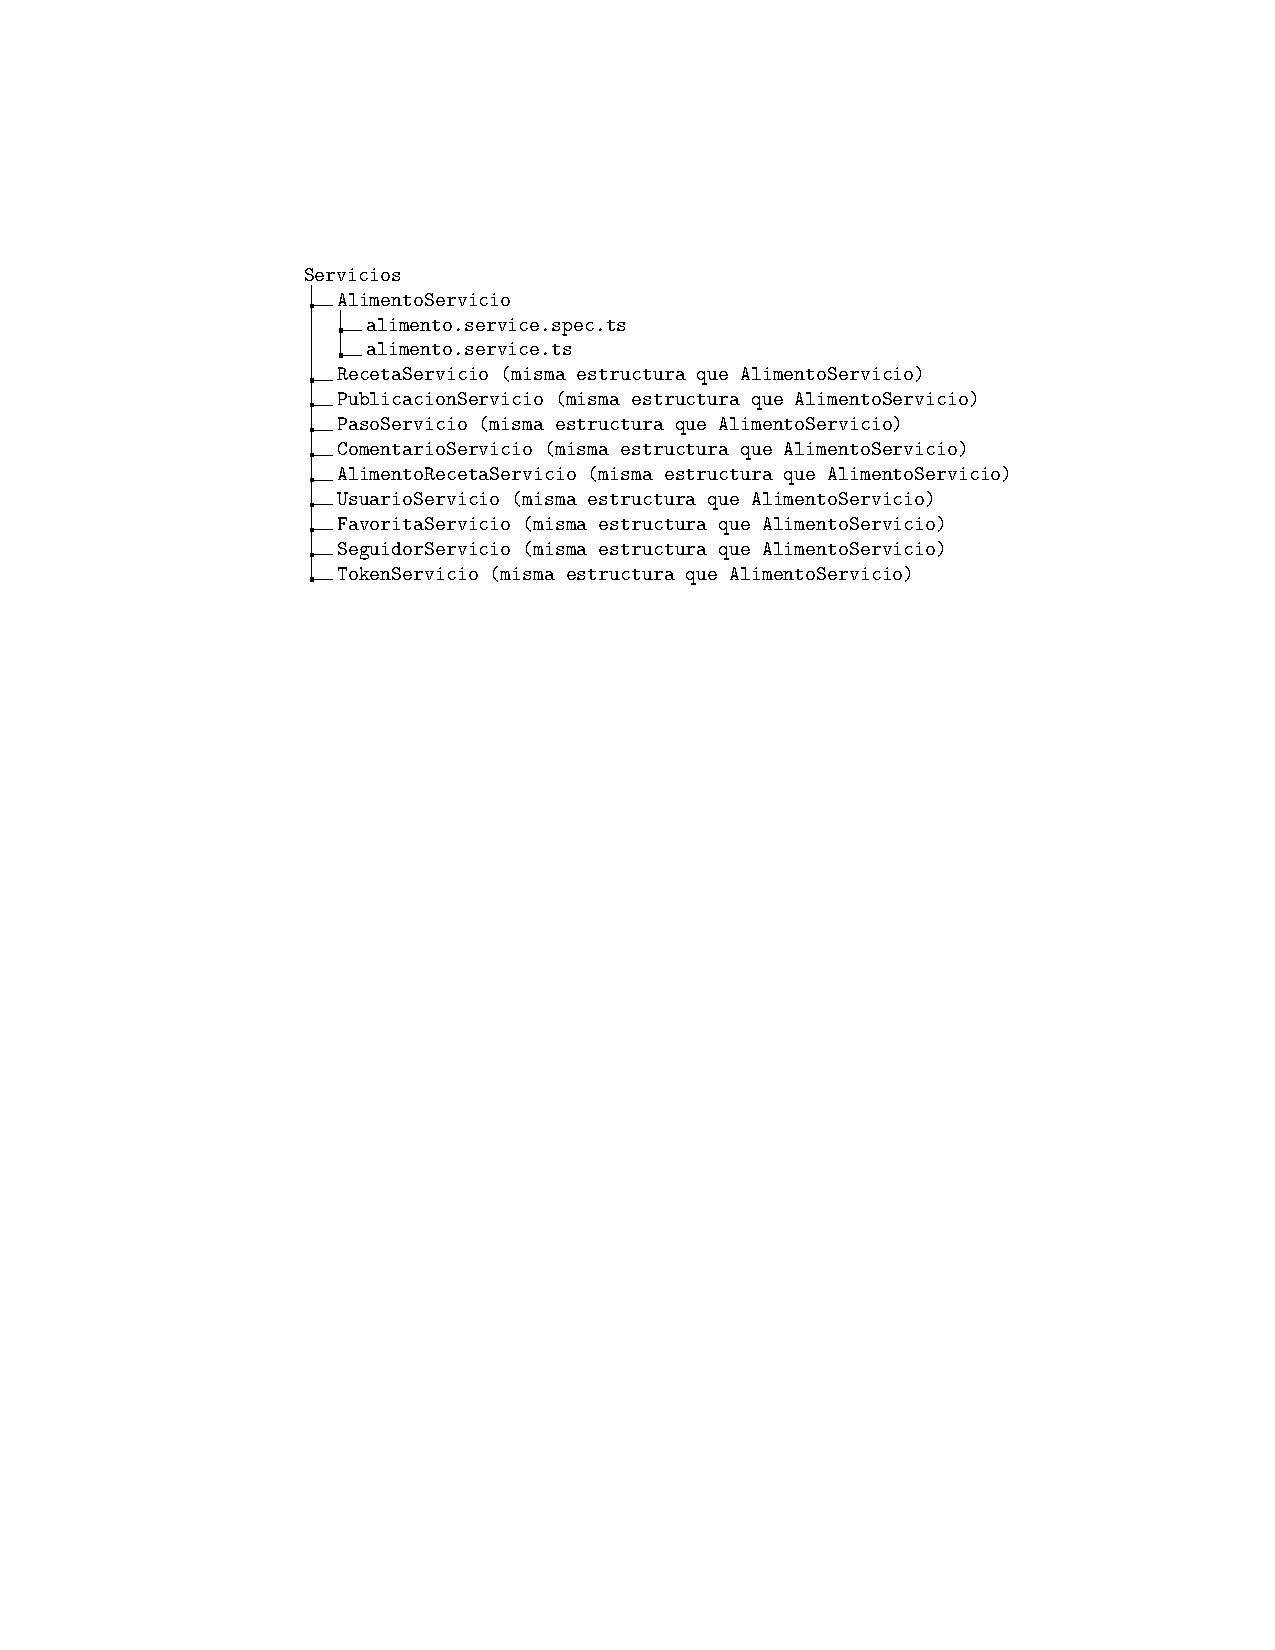
\includegraphics{img/dirtreeServicios.pdf}
    \caption{Estructura de ficheros en la carpeta \texttt{servicios}.}
    \label{fig:dirtreeServicios}
\end{figure}


En la Figura \ref{fig:dirtreeComponentes} se muestra la estructura de ficheros dentro de la carpeta \texttt{componentes}.

\begin{figure}
    \centering
    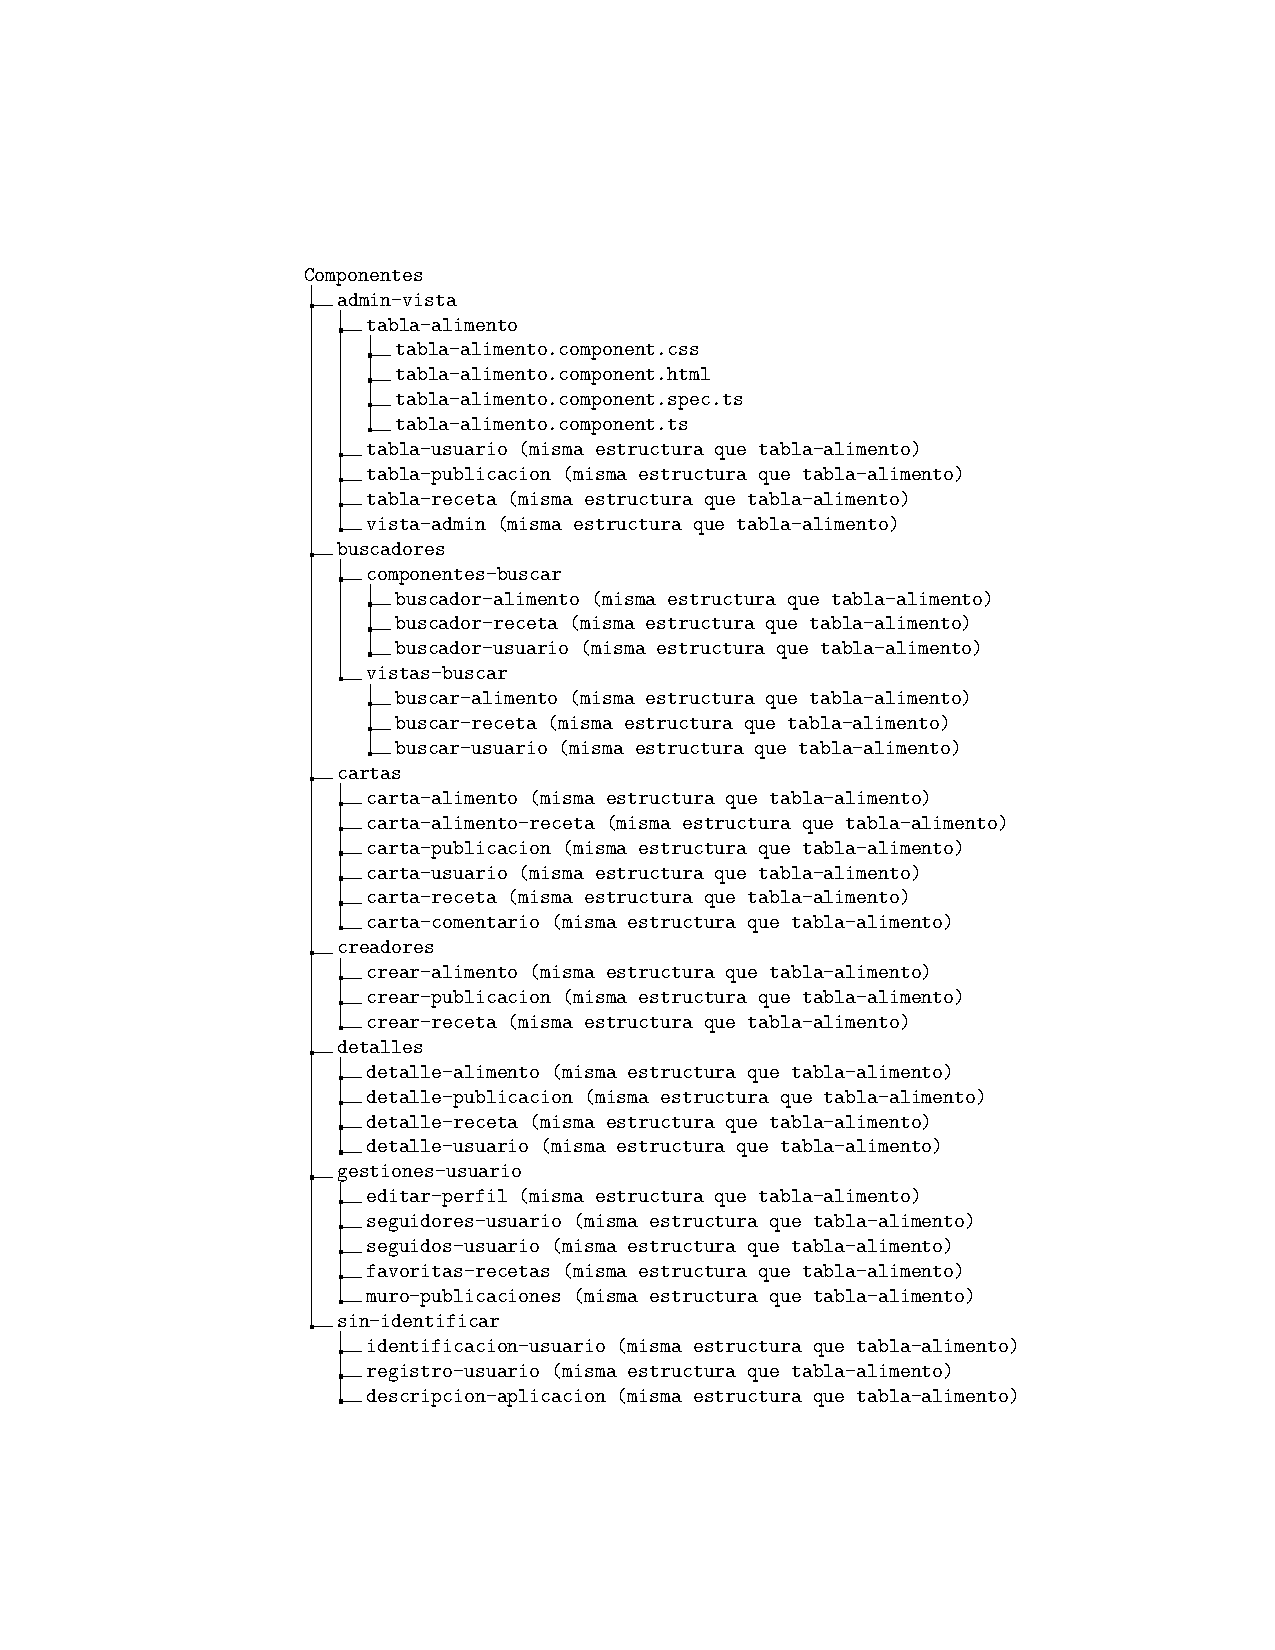
\includegraphics{img/dirtreeComponentes.pdf}
    \caption{Estructura de los ficheros en la carpeta \texttt{componentes}.}
    \label{fig:dirtreeComponentes}
\end{figure}






 

\section{Estructura del código de \textit{backend}}

En la Figura \ref{fig:dirtreeBack} se muestra la estructura de la parte realizada en NodeJS para el \textit{backend}.

\begin{figure}
    \centering
    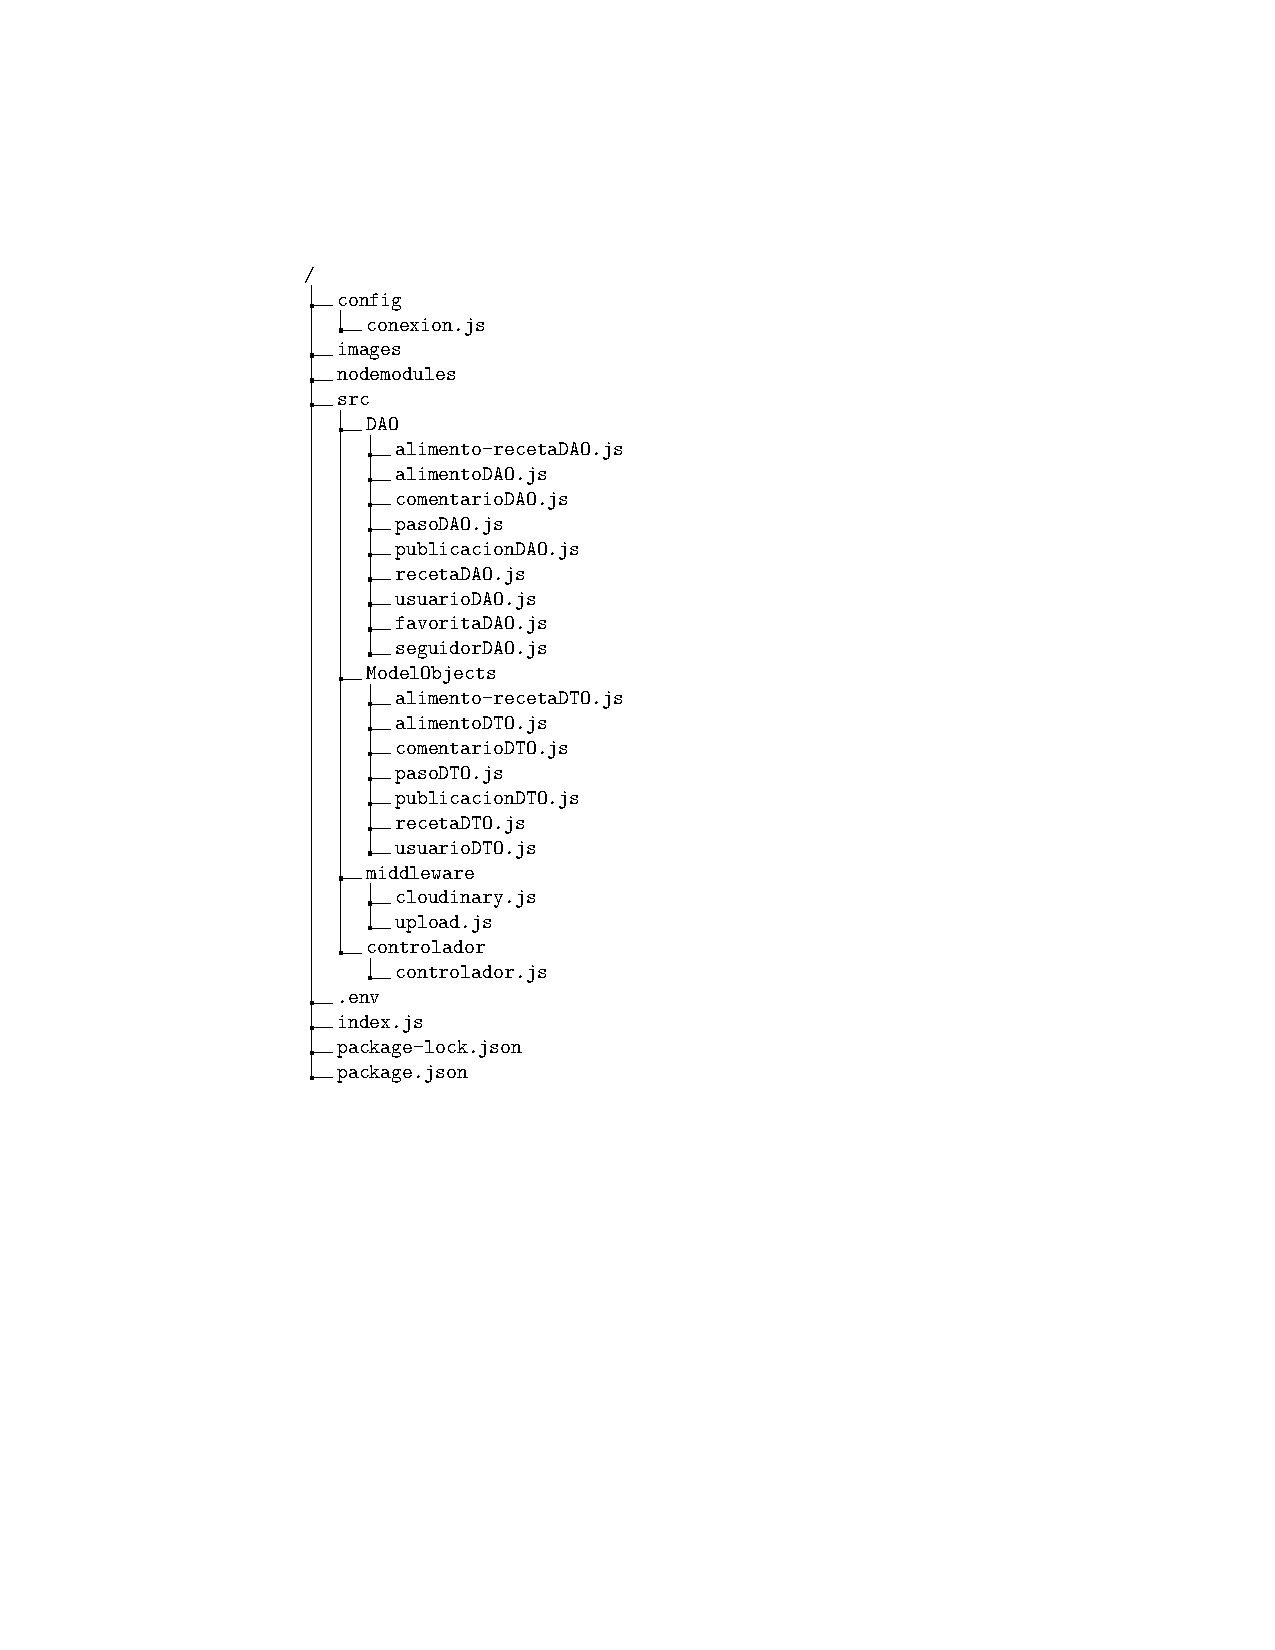
\includegraphics{svg/dirtreeback.pdf}
    \caption{Estructura de los ficheros en la parte del \textit{backend} en NodeJS.}
    \label{fig:dirtreeBack}
\end{figure}

A continuación se detalla el contenido de las carpetas y archivos mostrados en esta estructura:
\begin{itemize}
    \item Carpeta \texttt{config} que contiene el siguiente archivo:
    \begin{itemize}
        \item \texttt{config.js}: que se usa para la conexión con la base de datos SQL.
    \end{itemize}

    \item Carpeta \texttt{images}: se utiliza como carpeta auxiliar para guardar las imágenes temporalmente que suba el usuario.
    \item Carpeta \texttt{nodemodules}: contiene los paquetes instalados que se usan en NodeJS.
    \item Archivo \texttt{index.js}: es el archivo que se ejecuta para poner en funcionamiento esta parte del \textit{backend} de manera que empiece a escuchar peticiones en el puerto definido.
    \item Carpeta \texttt{src}: contiene el código principal de la parte de \textit{backend} y la descripción de las carpetas en su interior es la siguiente:
    \begin{itemize}
        \item \texttt{controlador}: esta carpeta contiene el siguiente archivo:
         \begin{itemize}
            \item \texttt{controlador.js}: en él se definen las rutas del \textit{backend} de la API REST a las que el \textit{frontend} puede realizar peticiones. Estas rutas se definen mediante el uso de ExpressJS y cada ruta llamará un método de un DAO de los almacenados en la carpeta \texttt{DAO} dependiendo de la operación solicitada y sobre qué tipo de datos se debe realizar.
        \end{itemize}
        
        
        \item \texttt{middleware}: en esta carpeta se encuentran los archivos que ayudan a almacenar las fotos que adjunte el Usuario a cada determinado tipo de datos. Estos archivos son los siguientes:
        \begin{itemize}
            \item \texttt{upload.js}: que almacena las fotos que adjunte el Usuario de manera temporal en la carpeta \texttt{images}.
            \item \texttt{cloudinary.js}: que se encarga de subir las fotos a Cloudinary para que queden almacenadas en la nube y se pueda acceder a ellas.
        \end{itemize}
        
    
        \item \texttt{DAO}: esta carpeta contiene los DAO para cada tipo de datos que se maneja en la aplicación. Cada DAO almacena las operaciones relacionadas sobre la base de datos para cada tipo de datos, de manera que en cada DAO se pueden encontrar agrupadas todas las operaciones sobre una determinada tabla de la base de datos.
        \item \texttt{ModelObjects}: esta carpeta contiene los DTO que se usarán para manejar los datos en el \textit{backend} que se obtengan de la base de datos y para enviárselos al \textit{frontend} en el formato correcto.
    \end{itemize}
\end{itemize}

       


\section{Pruebas}
Antes de que una aplicación Web sea utilizada por los clientes finales, es importante que sea verificada y validada a fondo para asegurarse de que todo funciona correctamente y de acuerdo a los objetivos de usuario. A continuación se definen los tipos de pruebas que se van a realizar:
\begin{itemize}
    \item \textbf{Prueba de funcionalidad:} estas pruebas comprueban que la aplicación Web se comporta según lo esperado sin problemas y la aplicación cumple con las especificaciones. Estas pruebas se encargan de comprobar la conexión entre el \textit{backend} y \textit{frontend}, los enlaces dentro de la aplicación Web y la información enviada u obtenida por el usuario. Son las principales para una aplicación Web porque verificarán si puede ejecutarse correctamente. Pueden realizarse manualmente o por un \textit{software} de prueba. La aplicación de estas pruebas a este proyecto se van a centrar en verificar que los enlaces funcionen correctamente y dirijan a la página deseada, que los formularios funcionen correctamente, verificando la validez de los campos introducidos por el usuario. Además, comprobarán que las \textit{cookies} almacenan los datos adecuados, que los archivos HTML y CSS del proyecto funcionan correctamente, que las interfaces se comportan como se espera y que el flujo de trabajo con la aplicación Web, es decir, como usaría la aplicación Web un Usuario final, funciona correctamente. Aquí es importante incluir escenarios inesperados de manera que la aplicación muestre los mensajes adecuados cuando el Usuario realice una acción que no es válida en la aplicación Web.
     
    \item \textbf{Pruebas de usabilidad:} estas pruebas sitúan la experiencia del Usuario en el centro de diseño de la aplicación. El objetivo principal de cualquier aplicación Web es atraer clientes, por lo tanto, estas pruebas se centran en comprobar como de fácil de utilizar es la aplicación Web. Estas pruebas se deben centrar en ver la facilidad con la que un Usuario puede navegar por la aplicación Web, si las funcionalidades que se ofrecen son fáciles de utilizar y si el contenido de la aplicación se muestra de una manera adecuada al Usuario para su uso. Para estas pruebas, la mejor opción es reclutar usuarios que puedan probar la aplicación definiendo ciertas acciones a realizar para comprobar si los usuarios pueden realizar lo que se pide. 
    
    \item \textbf{Pruebas de compatibilidad:} estas pruebas verifican que la aplicación sea compatible con todo tipo de dispositivos y navegadores. Para ello es importante verificar que la aplicación Web sea compatible con los principales navegadores como Google Chrome o Firefox, de manera que los usuarios puedan utilizar la aplicación en estos navegadores sin retrasos ni errores. Por otro lado, también es importante comprobar que la aplicación web funcione en todo tipo de sistemas operativos debido a la variedad de sistemas operativos que existen. Por último, pero un aspecto fundamental, es verificar que la aplicación sea compatible con todo tipo de dispositivos, de manera que funcione bien con todo tipo de tamaño de pantallas, debido a que cada Usuario utilizará un dispositivo diferente con un tipo  tamaño de pantalla único.
  
    
    
\end{itemize}

 Para las pruebas de funcionalidad, el propio desarrollador verificará que la aplicación se comporta como debe y cumple con las especificaciones. Para las pruebas de usabilidad se utilizarán usuarios cuyos perfiles sean similares a los perfiles de los usuarios finales de la aplicación para comprobar cómo se desenvuelven al utilizar la aplicación y si les resulta fácil utilizarla. Para las pruebas de compatibilidad, la aplicación se utilizará en diferentes navegadores, sistemas operativos y dispositivos para comprobar que en todos los casos funciona correctamente. 

\section{Problemas y dificultades encontradas}

A lo largo del desarrollo del proyecto se han ido encontrando diferentes problemas que han supuesto desafíos para la consecución con éxito del proyecto, pero finalmente se han podido encontrar solución a cada uno de ellos, aunque en cierta medida pueden haber retrasado el avance del proyecto. Los principales problemas afrontados han sido los siguientes:
\begin{itemize}
    \item \textbf{Almacenamiento de las fotos:} uno de los aspectos fuertes de cualquier aplicación es la capacidad que tiene el Usuario de adjuntar fotos para que el contenido que cree el Usuario sea más descriptivo. Para este proyecto este era también un aspecto importante y desde un primer momento, que se pudiesen adjuntar imágenes era un requisito indispensable para esta aplicación. Esta funcionalidad ha sido difícil de implementar debido a que hay variedad de opciones disponibles, cada una con sus ventajas y contras. La opción que se ha escogido es almacenar las fotos en la nube y guardar el enlace de acceso a cada foto en el objeto que tiene asociada esa foto en la base de datos, de manera que solo se necesite este enlace para acceder a la foto. 
    \item \textbf{Flujo de datos entre el \textit{frontend} y \textit{backend}:} la comunicación entre el \textit{backend} y el \textit{frontend} no ha sido sencilla de implementar debido a que las tablas almacenadas en la base de datos contenían numerosas relaciones lo que hacía que cada clase del Modelo de Dominio no contuviese toda la información relevante y se necesitasen de clases DTO con atributos añadidos para representar esta información. Este problema de comunicación entre el \textit{frontend} y \textit{backend} se ha resuelto utilizando clases DTO con atributos añadidos respecto a las clases del Modelo de Dominio para almacenar información relevante de las relaciones entre las tablas de la base de datos. Además se han utilizado consultas SQL complejas para obtener los datos necesarios.
     
    \item \textbf{Crecimiento de la aplicación y organización de su contenido:} este proyecto se divide en la parte de \textit{frontend} con Angular y la parte de \textit{backend} en NodeJS y ambas partes contienen gran cantidad de archivos de varios tipos agrupados en numerosas carpetas. En el momento que esta aplicación empezó a crecer en funcionalidad y el número de archivos que contenía empezó a aumentar, se volvió un aspecto fundamental organizar todos estos archivos en carpetas para que la aplicación pudiese seguir creciendo y se pudiese realizar la depuración de errores más fácilmente. 
\end{itemize}



\section{Casos de Prueba}

Las Tablas \ref{table:CP-01} a \ref{table:CP-23} muestran los casos de prueba. 

\begin{table}[H]
    \centering
    \begin{tabularx}{1\textwidth} { 
        | >{\raggedright\arraybackslash}X 
        | >{\raggedright\arraybackslash}X 
        | >{\raggedright\arraybackslash}X 
        |  }
    \hline
    \textbf{CP-01}     & \textbf{Iniciar sesión}                             \\ \hline
    Descripción        & El Usuario se identifica en la aplicación.      \\ \hline
    Entrada            &  \begin{itemize}
        \item \textit{username}: \textit{chema11}
        \item contraseña: \textit{123456789}
    \end{itemize}\\ \hline
    Escenario          & Introduce el \textit{username} y contraseña definido en la entrada y pulsa el botón \textit{identificarse}.                            \\ \hline
    Resultado esperado & El Usuario se ha identificado en la aplicación y se redirige a la vista \textit{muro-publicaciones}. \\ \hline
    Trazabilidad & CU-01 Iniciar sesión. \\ \hline
    \end{tabularx}
    \caption{CP-01. Iniciar sesión.}
    \label{table:CP-01}
    \end{table}

\begin{table}[H]
    \centering
    \begin{tabularx}{1\textwidth} { 
        | >{\raggedright\arraybackslash}X 
        | >{\raggedright\arraybackslash}X 
        | >{\raggedright\arraybackslash}X 
        |  }
    \hline
    \textbf{CP-02}     & \textbf{Registrarse}                             \\ \hline
    Descripción        & El Usuario se registra en la aplicación.      \\ \hline
    Entrada            & \begin{itemize}
        \item \textit{username}: \textit{chema99}
        \item contraseña: \textit{123456789}
        \item \textit{email}: \textit{chema99@gmail.com}
    \end{itemize}\\ \hline
    Escenario          & Introduce el \textit{username}, contraseña y \textit{email} definido en la entrada y pulsa el botón \textit{registrarse}.                            \\ \hline
   
    Resultado esperado & El Usuario se ha registrado en la aplicación y se redirige a la vista \textit{identificacion-usuario}. \\ \hline
    Trazabilidad & CU-02 Registrarse. \\ \hline
    \end{tabularx}
    \caption{CP-02. Registrarse.}
    \label{table:CP-02}
    \end{table}


   


        \begin{table}[H]
            \centering
            \begin{tabularx}{1\textwidth} { 
                | >{\raggedright\arraybackslash}X 
                | >{\raggedright\arraybackslash}X 
                | >{\raggedright\arraybackslash}X 
                |  }
            \hline
            \textbf{CP-03}     & \textbf{Cerrar sesión}                             \\ \hline
            Descripción        & El Usuario cierra su sesión en la aplicación.      \\ \hline
            
            Precondición          & El Usuario está identificado en el sistema.                             \\ \hline
            Escenario          & El Usuario pulsa el botón \textit{cerrar sesión}.                             \\ \hline
            Resultado esperado & El Usuario ha cerrado su sesión y se redirige a la vista \textit{identificacion-usuario}. \\ \hline
            Trazabilidad & CU-03 Cerrar sesión. \\ \hline
        \end{tabularx}
        \caption{CP-03. Cerrar sesión.}
        \label{table:CP-03}
            \end{table}


        \begin{table}[]
            \centering
            \begin{tabularx}{1\textwidth} { 
                | >{\raggedright\arraybackslash}X 
                | >{\raggedright\arraybackslash}X 
                | >{\raggedright\arraybackslash}X
                |  }
            \hline
            \textbf{CP-04}     & \textbf{Editar información del usuario}                             \\ \hline
            Descripción        & El Usuario edita la información de su cuenta.      \\ \hline
            Entrada            & \begin{itemize}
                \item foto: \textit{pruebas.jpg}
                \item contraseña: \textit{abcdefgh}
                \item \textit{email}: \textit{chema77@gmail.com}
                \item descripción: \textit{perfil de pruebas para la aplicación}
            \end{itemize} \\ \hline
            Escenario          & Introduce la foto, contraseña, \textit{email} y descripción definidas en la entrada y pulsa el botón \textit{editar perfil}.                            \\ \hline
            Precondición          & El Usuario está identificado en el sistema.                             \\ \hline
           
            Resultado esperado & El Usuario ha cambiado los datos de su cuenta y se redirige a la vista \textit{perfil-usuario}. \\ \hline
            Trazabilidad & CU-04 Editar información del Usuario. \\ \hline
        \end{tabularx}
        \caption{CP-04. Editar información del Usuario.}
        \label{table:CP-04}
            \end{table}

\clearpage

    \begin{table}[H]
        \centering
        \begin{tabularx}{1\textwidth} { 
            | >{\raggedright\arraybackslash}X 
            | >{\raggedright\arraybackslash}X 
            | >{\raggedright\arraybackslash}X 
            |  }
        \hline
        \textbf{CP-05}     & \textbf{Crear receta}                             \\ \hline
        Descripción        & El Usuario crea una receta.      \\ \hline
        Entrada            & \begin{itemize}
            \item título: \textit{receta de prueba}
            \item resumen: \textit{esta receta saludable sirve para probar la aplicación}
            \item tiempo: \textit{20}
            \item foto: \textit{pruebas.png}
            \item dificultad: \textit{fácil}
            \item pasos:
            \begin{itemize}
                \item \textit{Primero se ponen a cocer los macarrones}
                \item \textit{Después, se mezcla tomate con carne picada en una sartén}
                \item \textit{Finalmente se juntan los macarrones con el tomate y la carne picada}
            \end{itemize}
            \item alimentos en la receta:
            \begin{itemize}
                \item \textit{Macarrones, 300 gramos}
                \item \textit{Tomate, 200 gramos}
                \item \textit{Carne picada, 100 gramos}
            \end{itemize}
        \end{itemize} \\ \hline
        Escenario          & Introduce el título, resumen, tiempo, foto, dificultad, pasos y alimentos en la receta y pulsa el botón \textit{crear receta}.                           \\ \hline
        Precondición          & El Usuario está identificado en el sistema.                             \\ \hline
      
        Resultado esperado & El Usuario ha creado una receta y se redirige a la vista \textit{muro-publicaciones}. \\ \hline
        Trazabilidad & CU-06 Crear receta. \\ \hline
    \end{tabularx}
    \caption{CP-05. Crear receta.}
    \label{table:CP-05}
        \end{table}


\begin{table}[H]
    \centering
    \begin{tabularx}{1\textwidth} { 
        | >{\raggedright\arraybackslash}X 
        | >{\raggedright\arraybackslash}X 
        | >{\raggedright\arraybackslash}X
        |  }
    \hline
    \textbf{CP-06}     & \textbf{Ver publicaciones usuarios seguidos}                             \\ \hline
    Descripción        & El Usuario ve las publicaciones de los usuarios a los que sigue.      \\ \hline
    Entrada            & \begin{itemize}
        \item \textit{username}: \textit{chema11}
        \item contraseña: \textit{123456789}
    \end{itemize}  \\ \hline
    Escenario          & Introduce el \textit{username} y contraseña definidos en la entrada y pulsa \textit{identificarse} para iniciar sesión en la aplicación.                           \\ \hline
    Precondición          & El Usuario está identificado en el sistema.                             \\ \hline
   
    Resultado esperado & El Usuario se ha identificado en la aplicación y se redirige a la vista \textit{muro-publicaciones} donde se muestran las publicaciones de los usuarios a los que sigue. \\ \hline
    Trazabilidad & CU-05 Ver publicaciones usuarios seguidos. \\ \hline
\end{tabularx}
\caption{CP-06. Ver publicaciones usuarios seguidos.}
\label{table:CP-06}
    \end{table}


    \begin{table}[H]
        \centering
        \begin{tabularx}{1\textwidth} { 
            | >{\raggedright\arraybackslash}X 
            | >{\raggedright\arraybackslash}X 
            | >{\raggedright\arraybackslash}X 
            |  }
        \hline
        \textbf{CP-07}     & \textbf{Buscar alimento}                             \\ \hline
        Descripción        & El Usuario busca un alimento introduciendo su nombre.      \\ \hline
        Entrada            & \begin{itemize}
            \item nombre: \textit{brócoli}
        \end{itemize}\\ \hline
        Escenario          & Introduce el nombre del alimento definido en la entrada y pulsa el botón \textit{buscar}.                            \\ \hline
        Precondición          & El Usuario está identificado en el sistema.                             \\ \hline
        
        Resultado esperado & Se muestran todos los alimentos con un nombre similar al introducido por el usuario. \\ \hline
        Trazabilidad & CU-07 Buscar alimento. \\ \hline
    \end{tabularx}
    \caption{CP-07. Buscar alimento.}
    \label{table:CP-07}
        \end{table}


    \begin{table}[H]
        \centering
        \begin{tabularx}{1\textwidth} { 
            | >{\raggedright\arraybackslash}X 
            | >{\raggedright\arraybackslash}X 
            | >{\raggedright\arraybackslash}X
            |  }
        \hline
        \textbf{CP-08}     & \textbf{Buscar receta}                             \\ \hline
        Descripción        & El Usuario busca una receta introduciendo su título.      \\ \hline
        Entrada            & \begin{itemize}
            \item título: \textit{macarrones}
        \end{itemize} \\ \hline
        Escenario          & Introduce el título de la receta definido en la entrada y pulsa el botón \textit{buscar}.                            \\ \hline
        Precondición          & El Usuario está identificado en el sistema.                             \\ \hline
        
        Resultado esperado & Se muestran todas las recetas con un título similar al introducido por el usuario. \\ \hline
        Trazabilidad & CU-08 Buscar receta. \\ \hline
    \end{tabularx}
    \caption{CP-08. Buscar receta.}
    \label{table:CP-08}
        \end{table}


    \begin{table}[H]
        \centering
        \begin{tabularx}{1\textwidth} { 
            | >{\raggedright\arraybackslash}X 
            | >{\raggedright\arraybackslash}X 
            | >{\raggedright\arraybackslash}X 
            |  }
        \hline
        \textbf{CP-09}     & \textbf{Crear publicación}                             \\ \hline
        Descripción        & El Usuario crea una publicación.      \\ \hline
        Entrada            & \begin{itemize}
            \item título: \textit{publicación de prueba}
            \item descripción: \textit{esta publicación servirá para probar la aplicación}
            \item foto: \textit{pruebas.png}
            \item receta: \textit{macarrones con tomate}
        \end{itemize} \\ \hline
        Escenario          & Introduce el título, descripción, foto y receta definidos en la entrada y pulsa el botón \textit{crear publicación}.                            \\ \hline
        Precondición          & El Usuario está identificado en el sistema.                             \\ \hline
        
        Resultado esperado & El Usuario ha creado una publicación y se redirige a la vista \textit{muro-publicaciones}. \\ \hline
        Trazabilidad & CU-09 Crear publicación. \\ \hline
    \end{tabularx}
    \caption{CP-09. Crear publicación.}
    \label{table:CP-09}
        \end{table}


    \begin{table}[H]
        \centering
        \begin{tabularx}{1\textwidth} { 
            | >{\raggedright\arraybackslash}X 
            | >{\raggedright\arraybackslash}X 
            | >{\raggedright\arraybackslash}X 
            |  }
        \hline
        \textbf{CP-10}     & \textbf{Buscar Usuario}                             \\ \hline
        Descripción        & El Usuario busca un Usuario introduciendo su \textit{username}.      \\ \hline
        Entrada            & \begin{itemize}
            \item \textit{username}: \textit{javier89}
        \end{itemize} \\ \hline
        Escenario          & Introduce el \textit{username} definido en la entrada y pulsa el botón \textit{buscar}.                           \\ \hline
        Precondición          & El Usuario está identificado en el sistema.                             \\ \hline
       
        Resultado esperado & Se muestran todos los usuarios con un \textit{username} similar al introducido por el usuario. \\ \hline
        Trazabilidad & CU-10 Buscar Usuario. \\ \hline
    \end{tabularx}
    \caption{CP-10. Buscar usuario.}
    \label{table:CP-10}
        \end{table}


    \begin{table}[H]
        \centering
        \begin{tabularx}{1\textwidth} { 
            | >{\raggedright\arraybackslash}X 
            | >{\raggedright\arraybackslash}X 
            | >{\raggedright\arraybackslash}X
            |  }
        \hline
        \textbf{CP-11}     & \textbf{Consultar recetas favoritas}                             \\ \hline
        Descripción        & El Usuario consulta sus recetas marcadas como favoritas.      \\ \hline
        Escenario          & El Usuario pulsa el botón \textit{ver recetas favoritas}.                           \\ \hline
        Precondición          & El Usuario está identificado en el sistema.                             \\ \hline
        
        Resultado esperado & Se muestran las recetas marcadas como favoritas por el Usuario. \\ \hline
        Trazabilidad & CU-12 Consultar recetas favoritas.\\ \hline
    \end{tabularx}
    \caption{CP-11. Consultar recetas favoritas.}
    \label{table:CP-11}
        \end{table}


        \begin{table}[H]
            \centering
            \begin{tabularx}{1\textwidth} { 
                | >{\raggedright\arraybackslash}X 
                | >{\raggedright\arraybackslash}X 
                | >{\raggedright\arraybackslash}X
                |  }
            \hline
            \textbf{CP-12}     & \textbf{Borrar receta de favoritas}                             \\ \hline
            Descripción        & El Usuario elimina una receta de sus favoritas.      \\ \hline
            Escenario          & El Usuario pulsa el botón \textit{eliminar receta de favoritas}.                           \\ \hline
            Precondición          & El Usuario está identificado en el sistema.                             \\ \hline
            
            Resultado esperado & Se elimina la receta de las favoritas del usuario. \\ \hline
            Trazabilidad & CU-13 Borrar receta de favoritas.\\ \hline
        \end{tabularx}
        \caption{CP-12. Borrar receta de favoritas.}
        \label{table:CP-12}
            \end{table}


            \begin{table}[H]
                \centering
                \begin{tabularx}{1\textwidth} { 
                    | >{\raggedright\arraybackslash}X 
                    | >{\raggedright\arraybackslash}X 
                    | >{\raggedright\arraybackslash}X 
                    |  }
                \hline
                \textbf{CP-13}     & \textbf{Añadir receta a favoritas}                             \\ \hline
                Descripción        & El Usuario añade la receta a sus favoritas.      \\ \hline
                Escenario          & El Usuario pulsa el botón \textit{añadir receta a favoritas}.                            \\ \hline
                Precondición          & El Usuario está identificado en el sistema.                             \\ \hline
                
                Resultado esperado & Se añade la receta a las favoritas del usuario. \\ \hline
                Trazabilidad & CU-11 Añadir receta a favoritas.\\ \hline
            \end{tabularx}
            \caption{CP-13. Añadir receta a favoritas.}
            \label{table:CP-13}
                \end{table}



        \begin{table}[H]
            \centering
            \begin{tabularx}{1\textwidth} { 
                | >{\raggedright\arraybackslash}X 
                | >{\raggedright\arraybackslash}X 
                | >{\raggedright\arraybackslash}X
                |  }
            \hline
            \textbf{CP-14}     & \textbf{Consultar usuarios seguidos}                             \\ \hline
            Descripción        & El Usuario consulta sus usuarios seguidos.      \\ \hline
            Escenario          & El Usuario pulsa el botón \textit{ver usuarios seguidos}.                           \\ \hline
            Precondición          & El Usuario está identificado en el sistema.                             \\ \hline
            
            Resultado esperado & Se muestran los usuarios seguidos por el usuario. \\ \hline
            Trazabilidad & CU-14 Consultar usuarios seguidos.\\ \hline
        \end{tabularx}
        \caption{CP-14. Consultar usuarios seguidos.}
        \label{table:CP-14}
            \end{table}



            
        \begin{table}[H]
            \centering
            \begin{tabularx}{1\textwidth} { 
                | >{\raggedright\arraybackslash}X 
                | >{\raggedright\arraybackslash}X 
                | >{\raggedright\arraybackslash}X 
                |  }
            \hline
            \textbf{CP-15}     & \textbf{Dejar de seguir Usuario}                             \\ \hline
            Descripción        & El Usuario deja de seguir a un Usuario.      \\ \hline
            Escenario          & El Usuario pulsa el botón \textit{dejar de seguir usuario}.                           \\ \hline
            Precondición          & El Usuario está identificado en el sistema.                             \\ \hline
          
            Resultado esperado & El Usuario ya no sigue al Usuario. \\ \hline
            Trazabilidad & CU-15 Dejar de seguir Usuario.\\ \hline
        \end{tabularx}
        \caption{CP-15. Dejar de seguir Usuario.}
        \label{table:CP-15}
            \end{table}



            \begin{table}[H]
                \centering
                \begin{tabularx}{1\textwidth} { 
                    | >{\raggedright\arraybackslash}X 
                    | >{\raggedright\arraybackslash}X 
                    | >{\raggedright\arraybackslash}X 
                    |  }
                \hline
                \textbf{CP-16}     & \textbf{Seguir Usuario}                             \\ \hline
                Descripción        & El Usuario empieza a seguir a un Usuario.      \\ \hline
                Escenario          & El Usuario pulsa el botón \textit{seguir usuario}.                         \\ \hline
                Precondición          & El Usuario está identificado en el sistema.                             \\ \hline
                
                Resultado esperado & El Usuario seleccionado se añade a la lista de usuarios seguidos por el Usuario. \\ \hline
                Trazabilidad & CU-16 Seguir Usuario.\\ \hline
            \end{tabularx}
            \caption{CP-16. Seguir Usuario.}
            \label{table:CP-16}
                \end{table}


                \begin{table}[H]
                    \centering
                    \begin{tabularx}{1\textwidth} { 
                        | >{\raggedright\arraybackslash}X 
                        | >{\raggedright\arraybackslash}X 
                        | >{\raggedright\arraybackslash}X 
                        |  }
                    \hline
                    \textbf{CP-17}     & \textbf{Añadir comentario a publicación}                             \\ \hline
                    Descripción        & El Usuario añade un comentario a una publicación.      \\ \hline
                    Entrada            & \begin{itemize}
                        \item comentario: \textit{buena receta, tengo que probarla}
                    \end{itemize} \\ \hline
                    Escenario          & Introduce el comentario definido en la entrada y pulsa el botón \textit{guardar comentario}.                             \\ \hline
                    Precondición          & El Usuario está identificado en el sistema.                             \\ \hline
                    
                    Resultado esperado & El comentario se añade a la lista de comentarios de la publicación. \\ \hline
                    Trazabilidad & CU-17 Añadir comentario a publicación.\\ \hline
                \end{tabularx}
                \caption{CP-17. Añadir comentario a publicación.}
                \label{table:CP-17}
                    \end{table}



                    \begin{table}[H]
                        \centering
                        \begin{tabularx}{1\textwidth} { 
                            | >{\raggedright\arraybackslash}X 
                            | >{\raggedright\arraybackslash}X 
                            | >{\raggedright\arraybackslash}X 
                            |  }
                        \hline
                        \textbf{CP-18}     & \textbf{Eliminar Usuario}                             \\ \hline
                        Descripción        & El Administrador elimina un Usuario.      \\ \hline
                        Escenario          & El Administrador pulsa el botón \textit{eliminar usuario}.                           \\ \hline
                        Precondición          & El Administrador está identificado en el sistema.                             \\ \hline
                       
                        Resultado esperado & Se elimina el Usuario y todas sus publicaciones, recetas y comentarios creados. \\ \hline
                        Trazabilidad & CU-18 Eliminar Usuario.\\ \hline
                    \end{tabularx}
                    \caption{CP-18. Eliminar Usuario.}
                    \label{table:CP-18}
                        \end{table}


                \begin{table}[H]
                    \centering
                    \begin{tabularx}{1\textwidth} { 
                        | >{\raggedright\arraybackslash}X 
                        | >{\raggedright\arraybackslash}X 
                        | >{\raggedright\arraybackslash}X 
                        |  }
                    \hline
                    \textbf{CP-19}     & \textbf{Eliminar publicación}                             \\ \hline
                    Descripción        & El Administrador elimina una publicación.      \\ \hline
                    Escenario          & El Administrador pulsa el botón \textit{eliminar publicación}.                          \\ \hline
                    Precondición          & El Administrador está identificado en el sistema.                             \\ \hline
                  
                    Resultado esperado & Se elimina la publicación y todos sus comentarios. \\ \hline
                    Trazabilidad & CU-19 Eliminar publicación.\\ \hline
                \end{tabularx}
                \caption{CP-19. Eliminar publicación.}
                \label{table:CP-19}
                    \end{table}


            \begin{table}[H]
                \centering
                \begin{tabularx}{1\textwidth} { 
                    | >{\raggedright\arraybackslash}X 
                    | >{\raggedright\arraybackslash}X 
                    | >{\raggedright\arraybackslash}X 
                    |  }
                \hline
                \textbf{CP-20}     & \textbf{Eliminar alimento}                             \\ \hline
                Descripción        & El Administrador elimina un alimento.      \\ \hline
                Escenario          & El Administrador pulsa el botón \textit{eliminar alimento}.                            \\ \hline
                Precondición          & El Administrador está identificado en el sistema.                             \\ \hline
               
                Resultado esperado & Se elimina el alimento, todas sus publicaciones asociadas y todas las apariciones del alimento como ingrediente de una receta. \\ \hline
                Trazabilidad & CU-20 Eliminar alimento.\\ \hline
            \end{tabularx}
            \caption{CP-20. Eliminar alimento.}
            \label{table:CP-20}
                \end{table}


        \begin{table}[H]
            \centering
            \begin{tabularx}{1\textwidth} { 
                | >{\raggedright\arraybackslash}X 
                | >{\raggedright\arraybackslash}X 
                | >{\raggedright\arraybackslash}X 
                |  }
            \hline
            \textbf{CP-21}     & \textbf{Eliminar receta}                             \\ \hline
            Descripción        & El Administrador elimina una receta.      \\ \hline
            Escenario          & El Administrador pulsa el botón \textit{eliminar receta}.                          \\ \hline
            Precondición          & El Administrador está identificado en el sistema.                             \\ \hline
         
            Resultado esperado & Se elimina la receta, todas sus publicaciones asociadas y los alimentos definidos como ingredientes para su preparación. \\ \hline
            Trazabilidad & CU-22 Eliminar receta.\\ \hline
        \end{tabularx}
        \caption{CP-21. Eliminar receta.}
        \label{table:CP-21}
            \end{table}


            \begin{table}[H]
                \centering
                \begin{tabularx}{1\textwidth} { 
                    | >{\raggedright\arraybackslash}X 
                    | >{\raggedright\arraybackslash}X 
                    | >{\raggedright\arraybackslash}X 
                    |  }
                \hline
                \textbf{CP-22}     & \textbf{Crear alimento}                             \\ \hline
                Descripción        & El Administrador crea un alimento.      \\ \hline
                Entrada            & \begin{itemize}
                    \item nombre: \textit{macarrones}
                    \item descripción: \textit{pasta con muchos carbohidratos}
                    \item calorías: \textit{109}
                    \item foto: \textit{macarrones.jpg}
                    \item enlace: \textit{https://carrefour.es/macarrones1kg}
                    \item grasas: \textit{23}
                    \item carbohidratos: \textit{60}
                    \item proteínas: \textit{17}
                    \item cantidad: \textit{100}
                    \item medida: \textit{gramos}
                \end{itemize}\\ \hline
                Escenario          & Introduce el nombre, descripción, calorías, foto, enlace, grasas, carbohidratos, proteínas, cantidad y medida y pulsa el botón \textit{crear alimento}.                            \\ \hline
                Precondición          & El Administrador está identificado en el sistema.                             \\ \hline
               
                Resultado esperado & Se crea el alimento en la aplicación y el Usuario se redirige a la vista \textit{vista-admin}. \\ \hline
                Trazabilidad & CU-23 Crear alimento.\\ \hline
            \end{tabularx}
            \caption{CP-22. Crear alimento.}
            \label{table:CP-22}
                \end{table}


        \begin{table}[H]
            \centering
            \begin{tabularx}{1\textwidth} { 
                | >{\raggedright\arraybackslash}X 
                | >{\raggedright\arraybackslash}X 
                | >{\raggedright\arraybackslash}X 
                |  }
            \hline
            \textbf{CP-23}     & \textbf{Editar información de alimento}                             \\ \hline
            Descripción        & El Administrador edita la información de un alimento.      \\ \hline
            Entrada            & \begin{itemize}
                \item carbohidratos: \textit{70}
                \item grasas: \textit{13}
                \item foto: \textit{macarrones1.jpg}
            \end{itemize} \\ \hline
            Escenario          & Introduce los carbohidratos, grasas y foto y pulsa el botón \textit{editar alimento}.                            \\ \hline
            Precondición          & El Administrador está identificado en el sistema.                             \\ \hline
          
            Resultado esperado & Se actualizan los datos del alimento y el Administrador se redirige a la vista \textit{vista-admin}. \\ \hline
            Trazabilidad & CU-21 Editar información de alimento.\\ \hline
        \end{tabularx}
        \caption{CP-23. Editar información de alimento.}
        \label{table:CP-23}
            \end{table}
    



